\documentclass[sigplan,screen]{acmart}

\setcopyright{acmcopyright}
\copyrightyear{2018}
\acmYear{2018}
\acmDOI{10.1145/1122445.1122456}

\acmConference[REBLS '21]{REBLS '21: ACM Workshop on Reactive and Event-Based Languages and Systems}{June 03--05, 2018}{Chicago, IL}
\acmBooktitle{REBLS '21: ACM Workshop on Reactive and Event-Based Languages and Systems, June 03--05, 2018, Chicago, IL}
\acmPrice{15.00}
\acmISBN{978-1-4503-XXXX-X/18/06}

%\acmSubmissionID{123-A56-BU3}
%\citestyle{acmauthoryear}

\begin{document}

\title{Deterministic Distributed Interactive Applications}

\author{Francisco Sant'Anna}
\email{francisco@ime.uerj.br}
%\orcid{1234-5678-9012}
\affiliation{%
  \institution{Rio de Janeiro State University (UERJ)}
  \country{Brazil}
}

\author{Rodrigo Santos}
\email{rodrim.c@gmail.com}
\affiliation{%
  \institution{Microsoft}
  \country{Brazil}
}

\author{Noemi Rodriguez}
\email{noemi@inf.puc-rio.br}
\affiliation{%
  \institution{PUC-Rio}
  \country{Brazil}
}

%\renewcommand{\shortauthors}{Trovato and Tobin, et al.}

\begin{abstract}
A program is deterministic if re-execution with the same order of inputs always
leads to the same state.
It should even be possible to provide the same set of inputs to concurrent
instances in real time and observe identical behavior.
%
In this work, we guarantee real-time reproducibility in a distributed setting.
Mirrored instances of the same application are allowed to broadcast
asynchronous inputs and yet conform to identical behavior.
Collaborative networked applications, such as watch parties, document editing,
and video games can benefit of this approach.
%
Using a standard event-driven API to wait and generate events, programmers
write code as if the application executes in a single machine.
Our middleware intercepts event generation and synchronizes all instances so
that receipt is identically reproducible.
Not only distributed applications benefit of determinism but also development
and testing can be done in a single instance with the same guarantees.
\end{abstract}

\begin{comment}
\begin{CCSXML}
<ccs2012>
 <concept>
  <concept_id>10003033.10003083.10003095</concept_id>
  <concept_desc>Networks~Network reliability</concept_desc>
  <concept_significance>100</concept_significance>
 </concept>
</ccs2012>
\end{CCSXML}
\ccsdesc[100]{Networks~Network reliability}
\end{comment}

\keywords{globally-asynchronous locally-synchronous, synchronous programming}

\maketitle

\section{Introduction}

Deterministic programs are easier to understand, test, and verify~\cite{det}.
Considering user interactions, a program is deterministic if re-execution with
the same order and timing of inputs always leads to the same state.
With such reproducibility property, multiple re-executions are
indistinguishable from one another.
Considering now distribution, it should even be possible to provide the same
set of inputs to concurrent instances in real time and observe identical
behavior.

In this work, our goal is to guarantee real-time reproducibility property in a
distributed setting.
Mirrored instances of the same application running in different machines can
broadcast asynchronous inputs to each other and yet conform to
identical behavior.
Hence, our focus is on \emph{symmetric distributed applications}, instead of
machines playing different roles in the network.

Collaborative networked applications fall in the class of symmetric
distribution and can benefit of transparent determinism and reproducibility.
As an example, \emph{watch parties} are social gathering to watch movies and TV
shows.
Users expect to be perfectly synchronized such that anyone pressing the pause
button should stop all instances exactly in the same video frame.
In this context, the network and distance are just inconveniences that should
not make the experience to diverge from users sitting in front of the same TV.
Other examples that fall in this category are multiplayer games and
collaborative document editing.

Since our goal is to make distributed applications to \emph{behave} like local
applications, we also intend to make distributed programs to \emph{be coded}
like local programs.
In this sense, we provide a standard event-driven API with two main commands
to wait and generate events.
Programmers write the intended distributed application as if it would execute
in a single machine.
We also provide the middleware that connects the multiple application instances
transparently in the network.
The middleware intercepts event generation and synchronizes all instances so
that receipt is identically reproducible.
As a result, not only distributed applications benefit from determinism but
also development and testing can be done in a single instance with the same
guarantees.

As the main limitations, the middleware relies on a centralized server and all
instances must be known and responsive during the entire execution.
In addition, reaction to events takes the maximum round-trip time considering
all clients, which can be intolerable for low-latency applications such as
video games.

Section~\ref{sec.arch} describes the overall architecture of our middleware.
Section~\ref{sec.sync} discusses the synchronous programming model, which
programs following our event-driven API must comply in order to preserve
determinism.
Section~\ref{sec.gals} discusses the globally-asynchronous locally-synchronous
architecture of our middleware, and the synchronization algorithm to reproduce
the same set of inputs to all network instances in real time.
Section~\ref{sec.eval} evaluates our middleware with...
Section~\ref{sec.related}...
Section~\ref{sec.conclusion}...

\section{Overall Middleware Architecture}
\label{sec.arch}

Figure~\ref{fig.middleware} illustrates the client-server architecture of our
middleware entitled \emph{gals}.
A distributed application (\emph{dapp}, at the top left of the Figure), is a
set of mirrored instances running in different machines (also \emph{dapp},
inside the circles, to emphasize that they are symmetric and represent a single
application).
The clients, which are part of the middleware, intermediate all communication
with the server and empowers the \emph{dapp} instances to be specified as a
local application.
The server receives asynchronous events (in red) from the instances and is
responsible for redirecting them to all clients as synchronous events with an
appropriate delta delay (in green).
The clients control the clock ticks of the instances and is responsible for
issuing the received events at the appropriate timestamps.

\begin{figure}[t]
  \centering
  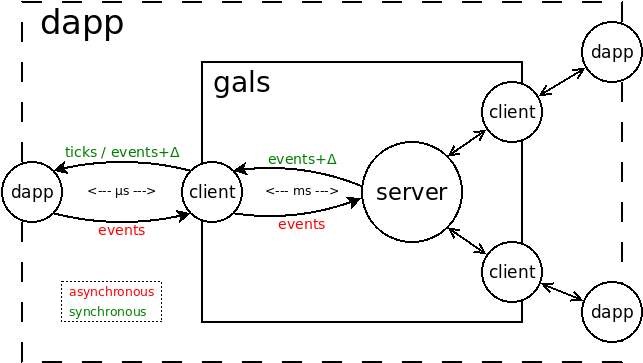
\includegraphics[width=\linewidth]{middleware}
  \caption{
    \label{fig.middleware}
    The architecture of the middleware \emph{gals}.
    A single server synchronizes multiple clients, each connected to a mirrored
    instance of the distributed application.
  }
  %\Description{A woman and a girl in white dresses sit in an open car.}
\end{figure}

The events represent user interactions, such as key presses, which are
unpredictable and need to be communicated with the other instances.
Since instances should be indistinguishable, event sources are irrelevant, at
least for theoretical purposes.
For instance, if a user presses a key in one instance, the \emph{dapp} behaves
as if all users pressed the same key at the same time.
%
Clock ticks represent the rate in which applications are updated, and are
equivalent to frame rates in video playback and games.
For practical purposes, we assume periods in the order of tens of milliseconds
(e.g., 25 milliseconds or 40 frames per second).
An important insight is that clock ticks are predictable inputs and need not to
go through the server.
This results in no delay between the \emph{dapp} and the client since
interprocess communication takes negligible time.
Unlike sporadic mechanical user input, clock ticks cannot accept delays in the
order of milliseconds without going unnoticed by humans.

As detailed in Section~\ref{sec.gals}, the delay for user input is the maximum
network round-trip time considering all clients.
Hence, the viability of the applications will depend on acceptable delay in the
user input and the maximum network latency.

Together with the 


symmetric distributed

  shows that ... but local
With distribution, communication timing is asynchronous because communication
latency takes a non-negligible time and breaks the synchronous hypothesis.


GALS...

Considering user interactions, a

 property
 with just two commands
 to broadcast
%
- not a equal apps, but the same app
    - one click in one is the same as in another, as if all xxx clicked together
Test locally in one instance is the same as N instances in M machines
What about in realtime
- a perfect mirror, cannot distinguish
- high-level vs low-leve events, semantic events

- transparent mechanism
- all network communication
- simple API
- clear/sound properties to reason
- no extra programming
- ressaltar questão da interatividade, inclusive no título
  - single application, multiple views, may restrict events per node

- reproduceable, but not in real-time since the environments are asynchronous

Concurrent programs in non-deterministic languages are notoriously hard to prove correct and have led to well-known disasters.


\section{Local Synchronous Programming}
\label{sec.sync}

In the synchronous programming model~\cite{sync}, a program executes in
locksteps (or logical ticks) as successive reactions to inputs provided by the
external environment.
The environment represents the user interacting with the application, and
inputs can be occasional events, such as a key press, or simply the passage of
time.
Since execution is guided from outside, the main advantage of the synchronous
model is that it can reproduce the exact behavior of a program by providing the
same sequence of inputs.
A fundamental requirement, known as the \emph{synchronous hypothesis}~\cite{hypo},
is that logical ticks are isolated from one another to preserve locksteps and
prevent concurrent reactions to inputs, which would break determinism.
This hypothesis is satisfied if computing reactions is faster than the rate of
external inputs.

An important concern is how to guarantee that isolated reactions are themselves
deterministic and sufficiently fast.
Synchronous languages~\cite{langs} typically restrict the programming
primitives and/or perform static analysis to ensure these properties.
Since our solution involves standard event-driven APIs for generic programming
languages, we assume these properties are met informally with coding best
practices, such as avoiding stateful system calls and time-consuming loops.

Synchronous: reactions run atomically and to comple-
tion on each line of execution, i.e., there’s no implicit
preemption or real parallelism.

Synchronous: reactions run atomically and to com-
pletion on each line of execution, i.e., there’s no
implicit preemption or real parallelism.

The synchronous execution model of Céu dictates
that reactions to input events are atomic and that in-
coming events are never lost, which we refer to as the
atomicity and responsiveness properties, respectively.

They rely on
the synchronous hypothesis which states that programs take no time to produce
outputs when reacting to inputs. The precise notion of time in these languages
is suitable for programming operations that should be performed respecting a
given timing constraint, which are common case in multimedia.

\section{GALS Architecture}
\label{sec.gals}

The ``Globally-Asynchronous Locally-Synchronous Architecture (GALS)''
integrates multiple independent synchronous processes as a single distributed
application.

\section{Evaluation}
\label{sec.eval}

\section{Related Work}
\label{sec.related}

Asynchronous languages and models:

Derflow: distributed deterministic dataflow programming for erlang
Erlang implements a message-passing execution model in which concurrent processes send each other messages asynchronously. This model is inherently non-deterministic: a process can receive messages sent by any process which knows its process identifier, leading to an exponential number of possible executions based on the number messages received. 
We propose a new execution model for Erlang, ''Deterministic Dataflow Programming'', based on a highly available, scalable single-assignment data store implemented on top of the riak\_core distributed systems framework.

Deterministic Actors
While actors provide a more disciplined model for concurrency than threads, their interactions, if not constrained, admit nondeterminism.
 We describe “reactors,” a new coordination model that combines ideas from several of the aforementioned approaches to enable determinism while preserving much of the style of actors.

Deterministic replay of distributed Java applications
Execution behavior of a Java application can be nondeterministic due to concurrent threads of execution, thread scheduling, and variable network delays. This nondeterminism in Java makes the understanding and debugging of multi-threaded distributed Java applications a difficult and a laborious process.
It is well accepted that providing deterministic replay of application execution is a key step towards programmer productivity and program under-standing.
Towards this goal, we developed a replay framework based on logical thread schedules and logical intervals.

Synchronous languages and models:

A Programming Model for Time-Synchronized Distributed Real-Time Systems
Discrete-event (DE) models are formal system specifications that have analysable deterministic behaviors. Using a global, consistent notion of time, DE components communicate via time-stamped events.
In this paper, we extend DE models with the capability of relating certain events to physical time.
Our technique relies on having a distributed common notion of time, known to some precision.

\section{Conclusion}
\label{sec.conclusion}

\bibliographystyle{ACM-Reference-Format}
\bibliography{rebls-21}

\end{document}
\endinput
